\documentclass{article}  % Define la clase del documento.

% Paquetes de idioma y codificación
\usepackage[utf8]{inputenc}
\usepackage[T1]{fontenc}
\usepackage[spanish]{babel}  % Ajusta el idioma del documento a español.

% Paquete de geometría para configurar márgenes y tamaño de papel
\usepackage[letterpaper, margin=3cm]{geometry}

% Paquetes de tipografía
\usepackage{mathptmx}    % Usa Times New Roman como fuente.
\usepackage{microtype}   % Mejora la justificación del texto.

% Paquetes para manejo de colores y gráficos
\usepackage{xcolor}      % Define y utiliza colores.
\usepackage{graphicx}    % Permite la inserción de imágenes.
\usepackage{tikz}        % Creación de gráficos vectoriales.

% Configuración de enlaces y referencias cruzadas
\usepackage{hyperref}
\hypersetup{
    colorlinks   = true,
    linkcolor    = darkblue,
    citecolor    = black,
    filecolor    = blue,
    urlcolor     = blue
}

% Paquetes para la mejora visual de tablas y figuras
\usepackage{booktabs}    % Para tablas de alta calidad.
\usepackage{float}       % Controla la posición de figuras y tablas.

% Paquete para la personalización de códigos fuente
\usepackage{listings}
\lstset{
    literate=
    {á}{{\'a}}1 {é}{{\'e}}1 {í}{{\'i}}1 {ó}{{\'o}}1 {ú}{{\'u}}1
    {Á}{{\'A}}1 {É}{{\'E}}1 {Í}{{\'I}}1 {Ó}{{\'O}}1 {Ú}{{\'U}}1
    {ñ}{{\~n}}1 {Ñ}{{\~N}}1 {ü}{{\"u}}1 {Ü}{{\"U}}1,
    backgroundcolor=\color{backcolour},
    commentstyle=\color{codegreen},
    keywordstyle=\color{codepurple},
    numberstyle=\tiny\color{codegray},
    stringstyle=\color{red},
    basicstyle=\ttfamily\small,
    breakatwhitespace=false,
    breaklines=true,
    captionpos=b,
    keepspaces=true,
    numbers=left,
    numbersep=5pt,
    showspaces=false,
    showstringspaces=false,
    showtabs=false,
    tabsize=2,
    language=TeX,
    morecomment=[l]\#,
    frame=single,
    rulecolor=\color{black}
}

% Definición de colores al estilo Visual Studio Code
\definecolor{darkblue}{rgb}{0.0, 0.0, 0.55}  % Enlaces
\definecolor{codegreen}{rgb}{0.25, 0.49, 0.48}  % Comentarios
\definecolor{codegray}{rgb}{0.5, 0.5, 0.5}  % Números y anotaciones
\definecolor{codepurple}{rgb}{0.58, 0, 0.82}  % Palabras clave
\definecolor{backcolour}{rgb}{0.95, 0.95, 0.92}  % Fondo de código

% Configuraciones de párrafo y matemáticas
\usepackage{amsmath}
\usepackage{parskip}    % Espaciado entre párrafos.
\usepackage{ragged2e}   % Justificación mejorada.

% Configuración de secciones y encabezados
\usepackage{titlesec}
\titleclass{\part}{top} % Make part like a class
\titleformat{\part}[display]
  {\normalfont\huge\bfseries\centering}{\thepart}{20pt}{\Huge}
\titlespacing*{\part}{172.5pt}{-60pt}{10pt}
\titleformat{\part}
  {\normalfont\huge\bfseries}{}{0pt}{}

% Asegúrate de usar esto para mantener el estilo en las páginas de las partes
\titleformat{\part}[display]
  {\normalfont\huge\bfseries}{}{0pt}{}
  [\thispagestyle{fancy}] % Aplica el estilo fancy a las páginas de las partes

% Configuración de encabezados y pies de página personalizados
\usepackage{fancyhdr}
\pagestyle{fancy}
\fancyhf{}
\fancyhead[L]{\raisebox{0.20cm}{\textbf{Apuntes Prueba 1 Hidrologia}}}
\fancyhead[R]{\raisebox{0.1cm}{
\includegraphics[width=0.25\linewidth]{LOGO_UNIVERSIDAD.jpg}}}
\fancyhead[C]{\rule{\textwidth}{0.6pt}}
\fancyfoot[C]{\rule{\textwidth}{0.6pt}}
\fancyfoot[R]{\raisebox{-1.5\baselineskip}{\thepage}}
\renewcommand{\headrulewidth}{0pt}
\renewcommand{\footrulewidth}{0pt}

% Configuración avanzada de geometría
\geometry{
  top=3.5cm, % Aumenta el espacio en la parte superior para subir el encabezado
  bottom=2.5cm,
  headheight=2.5cm % Aumenta la altura del encabezado si es necesario
}

% Configuracion de bibliografia
\usepackage{natbib}
\bibliographystyle{unsrtnat}  % Puedes cambiarlo por `unsrtnat`, `abbrvnat`, etc.

\begin{document}
%----------------------------------------------------------------------------------------
% PORTADA
%----------------------------------------------------------------------------------------
\begin{titlepage}%Inicio de la carátula, solo modificar los datos necesarios
\newcommand{\HRule}{\rule{\linewidth}{0.5mm}} 
\center 
%----------------------------------------------------------------------------------------
%	ENCABEZADO
%----------------------------------------------------------------------------------------

\includegraphics[width=10cm]{LOGO_UNIVERSIDAD.jpg}\\ % Si esta plantilla se copio correctamente, va a llevar la imagen del logo de la facultad.OBS: Es necesario incluir el paquete: graphicx
\vspace{3cm}
%----------------------------------------------------------------------------------------
%	SECCION DEL TITULO
%----------------------------------------------------------------------------------------
\HRule \\[0.4cm]
{ \huge \bfseries Apuntes Prueba 1}\\[0.4cm] % Titulo del documento
{ \huge \bfseries Hidrologia}\\[0.4cm] % Titulo del documento
\HRule \\[1.5cm]
 \vspace{5cm}
%----------------------------------------------------------------------------------------
%	SECCION DEL AUTOR
%----------------------------------------------------------------------------------------
\begin{flushright}
    { 
    \textbf{Autores:} \\
    Lukas Wolff Casanova\\
}
\end{flushright}
\vspace{1cm}
%----------------------------------------------------------------------------------------
%	SECCION DE LA FECHA
%----------------------------------------------------------------------------------------
{\large \textbf{\today}}\\[2cm] % El comando \today coloca la fecha del dia, y esto se actualiza con cada compilacion, en caso de querer tener una fecha estatica, reemplazar el \today por la fecha deseada
\end{titlepage}
%----------------------------------------------------------------------------------------
%  INDICE
%----------------------------------------------------------------------------------------
\newpage
\thispagestyle{empty} % Deshabilita el número de página en la página del índice
\tableofcontents
\thispagestyle{plain} % Deshabilita el encabezado en la página del índice
\thispagestyle{empty} % Deshabilita el número de página en la página del índice
\newpage

%\newpage
%\thispagestyle{empty}
%\listoffigures 
%\thispagestyle{plain} % Deshabilita el encabezado en la página del índice %
%\thispagestyle{empty}
%\newpage
%----------------------------------------------------------------------------------------
%ACÁ EMPIEZA EL INFORME
\setcounter{page}{1}
%----------------------------------------------------------------------------------------
\part{Capitulo 7}

\section{Tipos de Equipos}

\begin{itemize}
    \item Movimiento de Tierras
    \begin{itemize}
        \item Excavadoras (orugas con pala frontal)
        \item Buldozer
        \item Camion Tolva
        \item Retro Excavadora (Pala delantera y brazo atras)
        \item Mononiveladora (Niveladora de caminos)
        \item Motoniveladora (Igual pero con motor)
        \item Cargador Frontal (Pala frontal grande con articulacion en vehiculo y no en las ruedas)
        \item Mototrailla o Trailla (Permite ditribuir tierra)
    \end{itemize}
    \item Compactacion o Nivelacion
    \begin{itemize}
        \item Placa Compactadora (Se usa manualmente)
        \item Rodillo compactador liso (Hay de distintos tamaños)
        \item Rodillo compactador pata de cabra (Se usa para compactar mas profundamente)
        \item Rodillo compactador neumatico (Se usa para compactar asfalto, el que tiene muchas ruedas)
    \end{itemize}
    \item Produccion de Hormigon, existen distintos tipos de maquinas o instalaciones
\end{itemize}

\textbf{Criterios de Seleccion:} Se debe considerar el costo total, lo que comprende la inversion original mas el costo de operacion, costo de reparacion y mantencion del equipo. La suma de todo esto se define como \textbf{INVERSION TOTAL DE UN EQUIPO}

\section{Productividad de Equipos}

De este modo, se busca la productividad optima \textbf{Qp} la cual se basa en la operacion continua de la maquinaria por hora. Se define la productividad normal \textbf{Qv} como Qv incorporando el factor humano (0.85). Ademas si se agrega el factor de direccion del trabajo (fp), se optiene la productividad real \textbf{Qr}

\begin{equation}
    Qr = fp \cdot Qn = fp \cdot fw \cdot Qp = fa \cdot Qp
\end{equation}

\newpage
\section{Costos de Equipos}

Hay que tomar en consideracion costos como depreciacion e inversion inicial:

\begin{figure}[H]
    \centering
    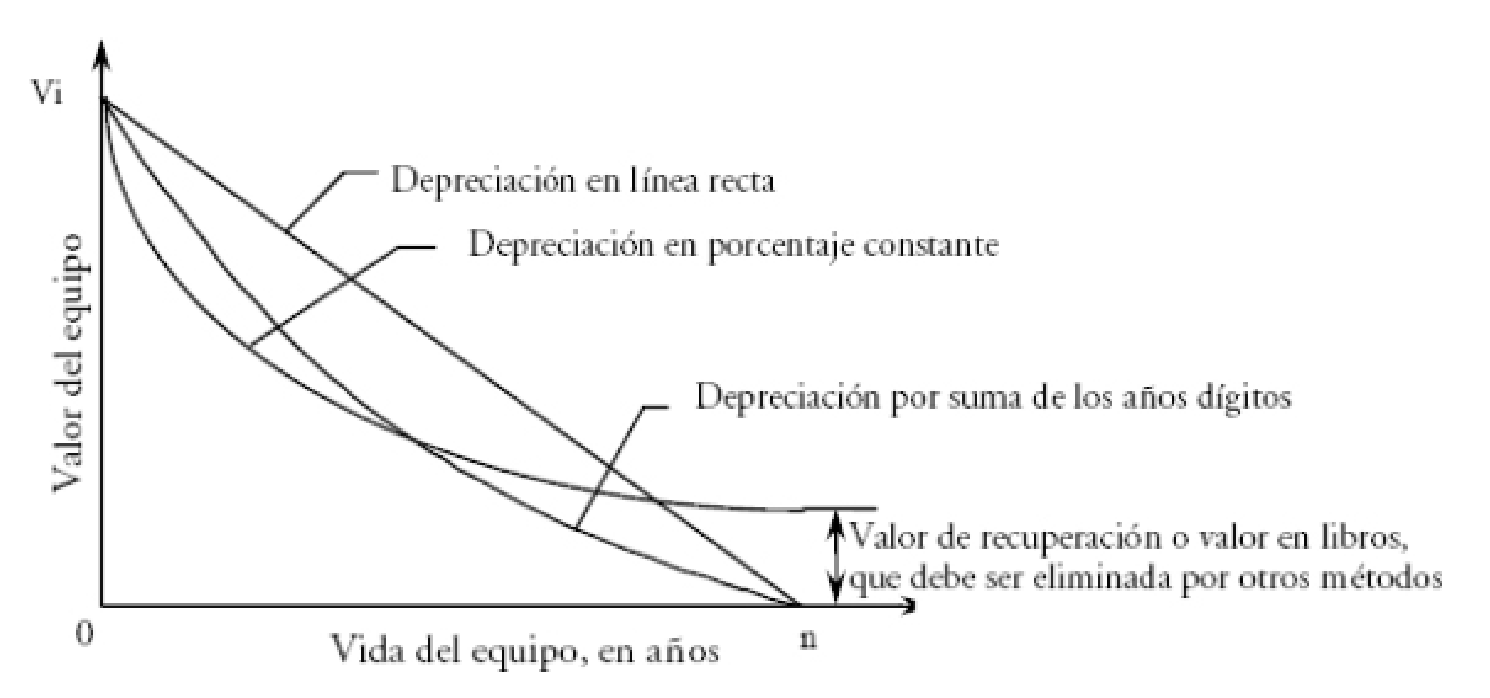
\includegraphics[width=0.8\linewidth]{FOTOS/costo_equipo.png}
    \caption{Costos de Equipos}
    \label{fig:costos}
\end{figure}

\begin{itemize}
    \item Costos de inversion
    \begin{itemize}
        \item Compra 
        \item Internacion
        \item Flete
        \item Seguro de traslado
        \item Intereses
        \item Impuestos
        \item Seguro
        \item Almacenaiento
    \end{itemize}
    \item Costos de operacion
    \begin{itemize}
        \item Operador
        \item Combustible
        \item Lubricacion
        \item mantencion
        \item Reparaciones menores
        \item Neumaticos y Filtros
    \end{itemize}
\end{itemize}

\newpage
\section{Vida Equipo}

De esta forma, la vida de un equipo se define como:

\begin{figure}[H]
    \centering
    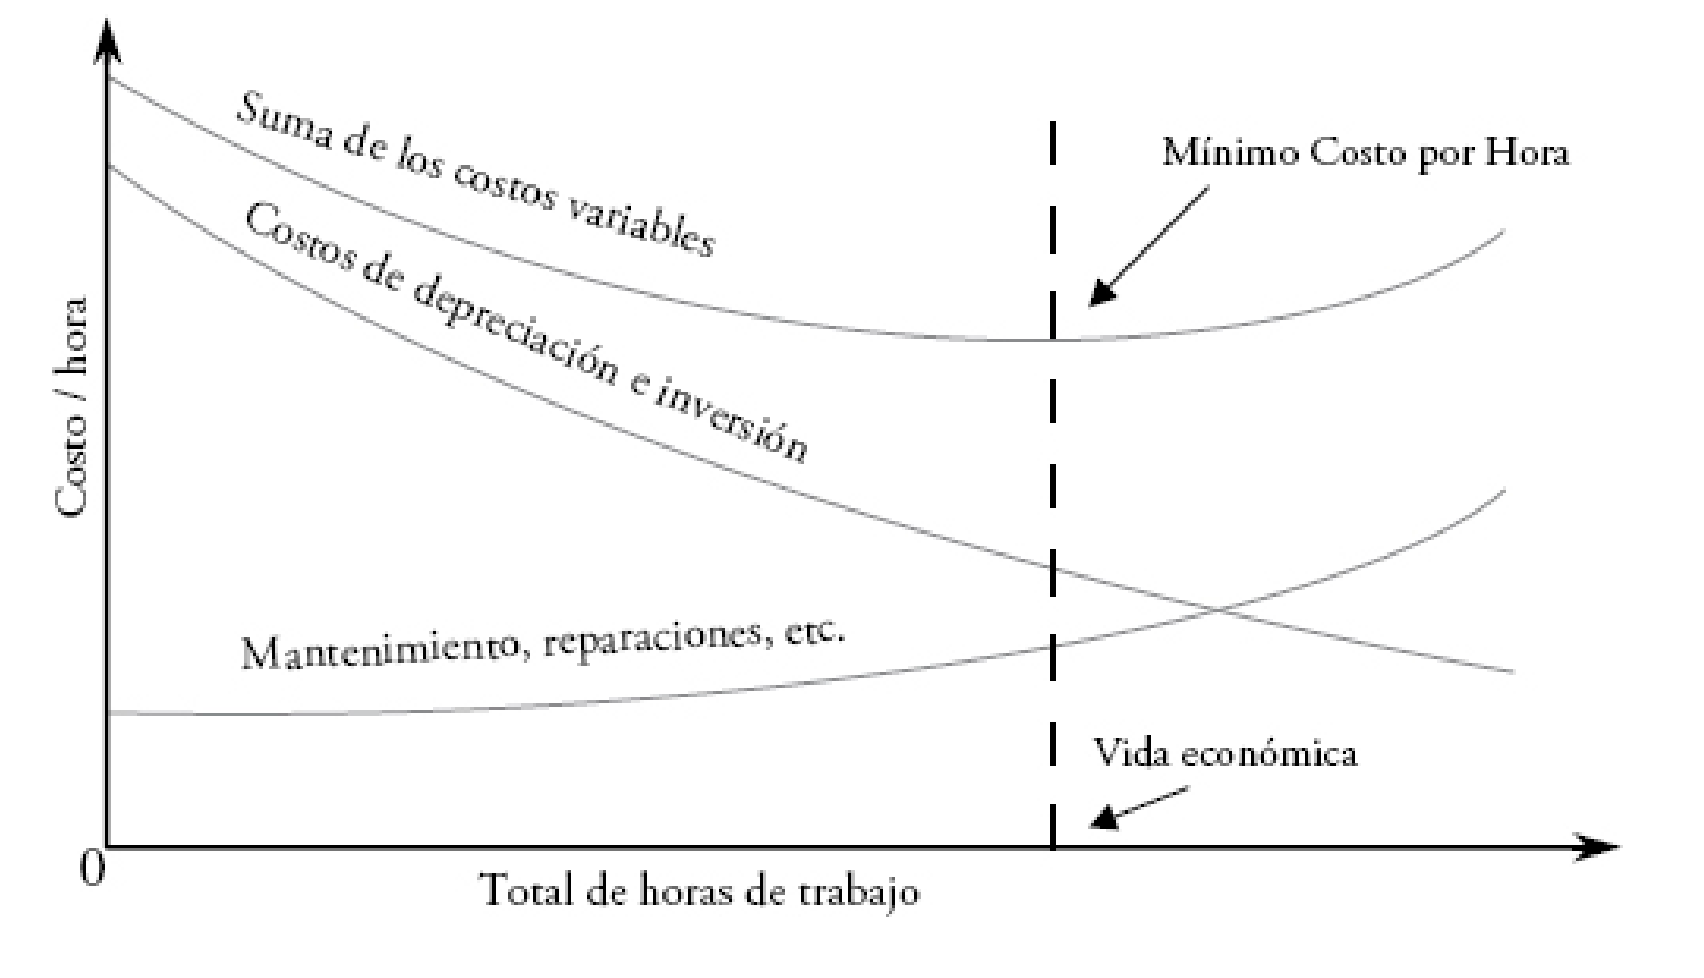
\includegraphics[width=0.8\linewidth]{FOTOS/vida_equipo.png}
    \caption{Vida de un Equipo}
    \label{fig:vida}
\end{figure}


\end{document}
